\subsection{Modelos de Phong y Blinn-Phong}
Empezamos viendo cómo las fuentes de luz presentes en la escena iluminan directamente la superficie. Hay multitud de modelos que simulan este comportamiento de forma más o menos realista, siendo uno de los más extendidos el renderizado basado en física (\textit{physically based rendering} o PBR). Sin embargo, este y otros acercamientos similares son utilizados cuando se requiere de un alto grado de fidelidad y adaptabilidad. Nosotros usaremos el modelo de reflexión de Blinn-Phong \cite{apuntes:ig}, también popular pero mucho más simple y computacionalmente menos costoso. A su vez este modelo se basa en el de Phong, presentado en 1975 \cite{phong}, y el cual pasamos a estudiar a continuación. \newline

Vamos a considerar que nuestra escena consta de los siguientes elementos.
\begin{itemize}
    \item La \textbf{isosuperficie} $S_{\phi}$ como único objeto a ser dibujado (aunque el modelo es válido para cualquier número de objetos en escena).
    \item Un \textbf{observador} que se encuentra en la posición $c_o\in\R^3$ mirando a un punto $p\in \R^3$.
    \item Un número finito $n$ de \textbf{fuentes de luz}. Llamaremos $l_i$ con $i\in \{1,\dots, n\}$ a los vectores normalizados que apuntan desde $p$ a la posición de cada fuente.
\end{itemize}

Empecemos comprendiendo el fenómeno físico que tratamos de simular. La luz que generan las fuentes no es más que radiación electromagnética. De forma ideal, esta radiación se puede ver como un flujo en el espacio de partículas llamadas \textbf{fotones} que siguen trayectorias rectilíneas a la par que interaccionan con el entorno. Cada una de estas partículas tendrá una energía radiante única en función de su longitud de onda, que irá transfiriendo a aquellos objetos con los que interaccione.

\begin{definicion}[Radiancia]
    Dado un punto $p\in\R^3$, llamamos \textbf{radiancia} a la densidad de energía radiante por unidad de tiempo de los fotones que pasan por un entorno de $p$ en una determinada dirección $v\in\R^3$ con $\Vert v\Vert = 1$. La denotaremos $L(p,v)$, y será representada mediante una terna RGB no acotada. Podemos distinguir a su vez varios tipos de radiancia.
    \begin{itemize}
        \item \textbf{Radiancia emitida $\boldsymbol{L_E(p,v)}$:} radiancia que emite el propio objeto, también llamada emisividad. Normalmente es de intensidad baja y la consideraremos constante.
        \item \textbf{Radiancia incidente $\boldsymbol{L_{I}}(p,v)$:} radiancia que recibe el punto $p$ desde la dirección $v$. 
        \item \textbf{Radiancia reflejada $\boldsymbol{L_{R}}(p,v)$:} cantidad de la radiancia incidente en $p$ que se refleja en la dirección $v$. 
\end{itemize}
\end{definicion}

El objetivo del modelo será por tanto describir la radiancia que percibe el observador desde su posición en el punto $p$. Para ello, se llevan a cabo una serie de simplificaciones:
\begin{itemize}
    \item En un modelo físicamente correcto la luz reflejada en cada punto se dispersaría por el entorno, contribuyendo a la radiancia incidente en otros puntos de la escena. Sin embargo, nosotros no consideraremos la radiancia incidente que no provenga directamente de fuentes de luz. Incluso teniendo un solo objeto en escena como es nuestro caso este modelo es mejorable, pues el objeto puede reflejar radiancia sobre sí mismo. Por tanto, usaremos una radiancia ambiente constante $L_A$ para suplir esta iluminación indirecta.
    \item La radiancia se conserva en el espacio entre objetos.
    \item Las fuentes de luz son direccionales, de forma que no serán visibles en la escena. Además supondremos que emiten una radiancia constante $S_i$ para $i\in \{1,\dots, n\}$.
    \item No se consideran objetos con transparencia.
\end{itemize}
Es natural pensar que la radiancia percibida en un punto $p\in \R^3$ será la suma de la radiancia que emita y la que sea capaz de reflejar. Así, teniendo en cuenta las consideraciones anteriores tenemos que
\begin{equation*}
    L(p,v) = L_A + L_E + \sum_{i=1}^n L_R(p,l_i).
\end{equation*}
Como $L_A$ y $L_E$ son constantes solo nos falta estudiar cómo obtener la \textbf{radiancia reflejada} para cada fuente de luz. Para ello fijamos un índice $m\in \{1,\dots,n\}$ y suponemos a partir de ahora que $p\in S_{\phi}$ ya que, si bien la radiancia en un punto $q\notin S_{\phi}$ en la dirección $v$ depende de la radiancia saliente del primer punto visible desde $q$ en la dirección $-v$, nosotros solo evaluaremos el modelo de iluminación cuando detectemos una intersección con la superficie. En caso de no hallar intersección alguna tomaremos simplemente
\begin{equation*}
    L(p,v) = L_A,\ p\notin S_{\phi}.
\end{equation*}

Sabemos que cada objeto refleja la luz de manera distinta en función de su material y las propiedades de la fuente. Para representar este comportamiento definimos una función que indique la fracción de radiancia proveniente de la $m$-ésima fuente de luz visible desde $p$ en la dirección $l_m$ que se refleja en un punto $p$ en la dirección $v$ para cada fuente de luz
\begin{equation*}
    f_r \colon \R^3\times \R^3\times \R^3 \to \R^3.
\end{equation*}
Así, la radiancia reflejada es
\begin{equation*}
    L_R(p,v,l_m) = S_m\cdot f_r(p,v,l_m).
\end{equation*}

Podemos distinguir diferentes tipos de reflexión, cada uno contribuyendo de forma diferente a la radiancia reflejada final.

% donde $f_a$, $f_d$ y $f_e$ representan la fracción de radiancia reflejada para cada uno de los tipos de reflexión que podemos distinguir y listamos a continuación. 
\begin{itemize}
    \item \textbf{Reflexión ambiental:} cantidad de iluminación indirecta proveniente de la fuente de luz que refleja el objeto. Al igual que hicimos con $L_A$, tomaremos un valor constante $R_A$ para ella, de forma que la fracción de radiancia ambiental reflejada será
    \begin{equation*}
        f_{ra} =  R_A \in \R^3.
    \end{equation*}
    \item \textbf{Reflexión especular:} define cómo se refleja la luz en objetos brillantes teniendo en cuenta la posición de la fuente de luz y la del observador. Según la ley de reflexión, el ángulo de incidencia de la luz será igual al de reflexión, luego podemos obtener la dirección de reflexión $r_m$ reflejando $l_m$ sobre el vector normal unitario en $p$ de la superficie, que llamaremos $N_p$. De esta forma, tenemos que
    \begin{equation*}
        r_m = 2(l_m\cdot N_p)N_p - l_m \in \R^3.
    \end{equation*}

    Sin embargo, solo queremos que haya reflejos en los puntos orientados hacia la fuente de luz y cuando $r_m$ haya sido reflejado en una dirección que el observador pueda apreciar, siendo la intensidad del reflejo mayor cuanto más alineado esté el observador con el vector reflejado. Esto equivale a que se cumpla
    \begin{equation*}
        N_p\cdot l_m >0 \quad \text{ y }\quad  R_m \cdot v>0.
    \end{equation*}
    Para controlar el color y la intensidad de los reflejos usaremos un factor $R_E$ que codifique la fracción de radiancia reflejada de esta forma, de modo que podemos expresar la fracción de radiancia especular reflejada como
    \begin{align*}
        f_{re} \colon \R^3\times \R^3\times \R^3 &\to \R^3,\\
        (p,v,l_m) &\mapsto R_E \cdot \Max(0,r_m \cdot v)^{\alpha},\ \alpha\in \R.
    \end{align*}
    El valor $\alpha$ se llama \textbf{exponente de brillo}, y nos proporciona control sobre el tamaño e intensidad de las zonas brillantes del objeto, siendo más pequeños e intensos los brillos generados cuanto mayor sea su valor. Un ejemplo de por qué esto nos resulta útil es comparar materiales especulares, como el mármol y el metal. Ambos generan brillos sobre su superficie, pero en el caso del metal estos son más pequeños y brillantes debido a que se trata de un material más pulido, luego tomaríamos $\alpha_{metal} > \alpha_{m\acute{a}rmol}$. 
    \item \textbf{Reflexión difusa:} modela cómo se refleja la luz en objetos mates en función de la posición de la fuente de luz. Al contrario de lo que ocurre con la reflexión especular, debido a la irregularidad de la superficie del objeto la luz no se refleja en una sola dirección, haciendo que se disperse en direcciones impredecibles. Este comportamiento se simula a través de una radiancia $R_D$ que represente el valor promedio resultado de estos reflejos, y que consideraremos constante. Un ejemplo de material con estas propiedades sería el yeso, para el cual tomaríamos $\Vert R_D\Vert \gg \Vert R_E\Vert$.  Al igual que antes, solo queremos que el punto esté iluminado cuando esté de cara a la fuente de luz, obteniendo la mayor cantidad de luz cuando está alineado con la fuente. Así, la fracción de radiancia difusa será
    \begin{align*}
        f_{rd} \colon \R^3\times \R^3\times \R^3 &\to \R^3,\\
        (p,v,l_m) &\mapsto R_D\cdot \Max(0,l_m \cdot N_p).
    \end{align*}
\end{itemize}

\begin{figure}[!h]
    \centering
    \begin{subfigure}[b]{0.25\textwidth}
        \centering
        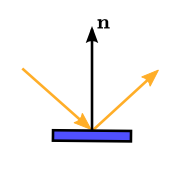
\includegraphics[width=\textwidth]{Plantilla-TFG-master/img/glossyTodiffuse1.png}
        \caption{Especular perfecta}
    \end{subfigure}
    \hfill
    \begin{subfigure}[b]{0.48\textwidth}
        \centering
        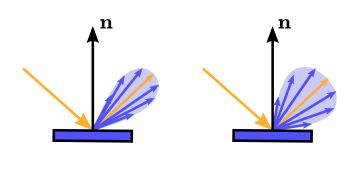
\includegraphics[width=\textwidth]{Plantilla-TFG-master/img/glossyTodiffuse2.png}
        \caption{Pseudo-especulares}
    \end{subfigure}
    \hfill
    \begin{subfigure}[b]{0.20\textwidth}
        \centering
        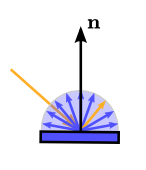
\includegraphics[width=\textwidth]{Plantilla-TFG-master/img/glossyTodiffuse3.png}
        \caption{Difusa}
    \end{subfigure}
    \hfill
    \caption{Tipos de función de distribución de reflexión bidireccional \cite{especular}}
\end{figure}

\begin{observacion}
    Es necesario que los vectores $l_i$, $v$ y $N_p$ sean unitarios, pues de lo contrario su producto escalar no coincidiría con el coseno del ángulo que forman.
\end{observacion}

% En vista de las definiciones anteriores, podríamos simplemente definir
% \begin{equation*}
%     f_r(p,v,l_m) = f_{ra}+f_{re}(p,v,l_m) + f_{r_d}(p,v,l_m).
% \end{equation*}

% De esta forma, para diferenciar entre un material totalmente mate como el yeso y uno especular como el metal bastaría tomar valores de $R_D$ y $R_E$ tal que $\Vert R_D\Vert \gg \Vert R_E\Vert$. Sin embargo, a la hora de comparar materiales especulares podríamos observar que aunque ambos generen zonas brillantes no lo hagan de la misma forma. Por ejemplo, tanto el mármol como el metal generan brillos sobre su superficie, pero en el caso del metal estos son más pequeños y brillantes debido a que se trata de un material más pulido. Por tanto, para añadir control sobre el tamaño e intensidad de estas zonas brillantes introducimos el \textbf{coeficiente de brillo} $\alpha \in \R$ en la expresión de $f_{re}$, de forma que cuanto mayor sea su valor más pequeños e intensos serán los brillos generados. En la \autoref{fig:parametrosEspecular} podemos ver el efecto que tienen $R_E,R_D$ sobre la radiancia reflejada \cite{especular}.\newline

\begin{definicion}
    Dado un objeto, definimos su \textbf{material} como la tupla $\{R_A,R_E,R_D,\alpha \}$.
\end{definicion}

Una vez asociado un material a $S_{\phi}$ podemos escribir la expresión final para $f_r$:

\begin{align}\label{eq:fr}
    f_r(p,v,l_i) &= f_{ra} &+\ & f_{re}(p,v,l_i) &+\ &f_{r_d}(p,v,l_i)\\
                 &= R_A    &+\ & R_E \cdot \Max(0,r_i \cdot v)^{\alpha} &+\  &R_D\cdot \Max(0,l_i\cdot N_p). 
\end{align}

\begin{figure}[!h]
     \begin{subfigure}[b]{0.45\linewidth}
        \centering
        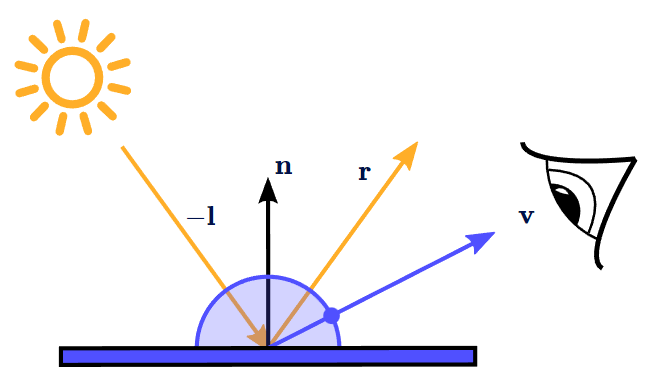
\includegraphics[width=0.95\textwidth]{Plantilla-TFG-master/img/ks0kd1.png}
        \caption{$\Vert R_E\Vert = 0$}
     \end{subfigure}
     \hfill
     \begin{subfigure}[b]{0.45\linewidth}
        \centering
        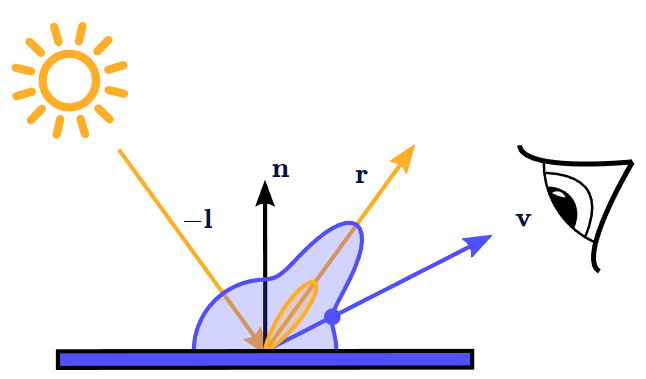
\includegraphics[width=0.95\textwidth]{Plantilla-TFG-master/img/ks1kd1.png}
        \caption{$\Vert R_E\Vert =\Vert R_D\Vert$ y $\alpha$ grande}
     \end{subfigure}
     \hfill
     \begin{subfigure}[b]{0.45\linewidth}
        \centering
        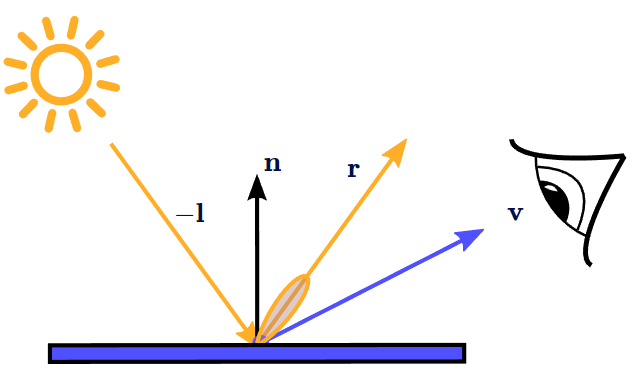
\includegraphics[width=0.95\textwidth]{Plantilla-TFG-master/img/ks1kd0.png}
        \caption{$\Vert R_D\Vert = 0$ y $\alpha$ grande}
     \end{subfigure}
     \hfill
     \begin{subfigure}[b]{0.45\linewidth}
        \centering
        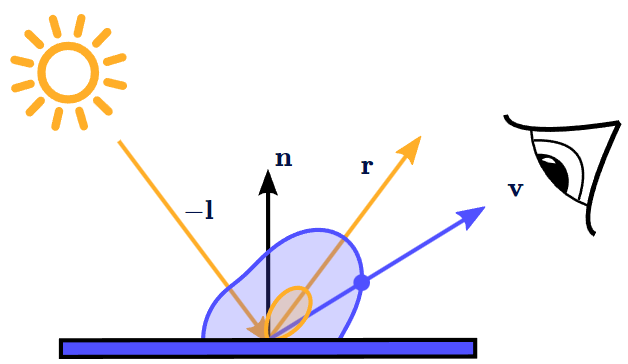
\includegraphics[width=0.95\textwidth]{Plantilla-TFG-master/img/ks1kd1a0.png}
        \caption{$\Vert R_E\Vert =\Vert R_D\Vert$ y $\alpha$ pequeño}
     \end{subfigure}
     % \begin{minipage}[c]{0.45\linewidth}
     %    \centering
     %    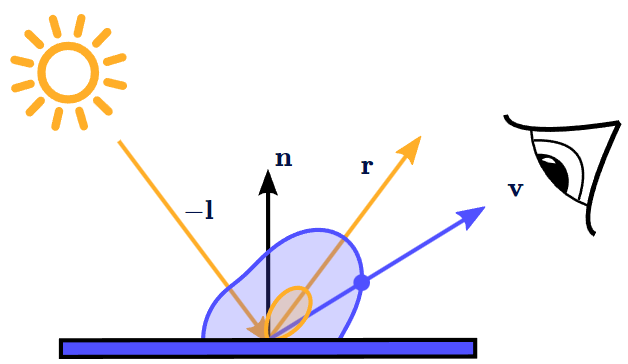
\includegraphics[width=0.95\textwidth]{Plantilla-TFG-master/img/ks1kd1a0.png}
     %    \caption{$k_s = 1$ y $k_d = 0$}
     % \end{minipage}
     \caption{Ejemplo de distintos valores para $R_E,R_D$ y $\alpha$}
     \label{fig:parametrosEspecular}
\end{figure}

Recogemos los resultados obtenidos en la siguiente definición.
\begin{definicion}[Modelo de Phong]\label{def:blinn} La radiancia percibida en el punto $p\in\R^3$ desde la dirección $v\in\R^3$ con $\Vert v\Vert = 1$ según el modelo de Phong viene dada por
    \begin{equation*}
        L(p,v) = L_A+L_E+ \sum_{i=0}^n S_i \Bigg[ R_A + R_E\cdot \Max(0,r_i\cdot v)^{\alpha} + R_D\cdot \Max(0,l_i\cdot N_p) \Bigg],
    \end{equation*}

    donde:
    \begin{itemize}
        \item $n \in \N$ es el número de fuentes de luz y $l_i \in R^3$ es el vector normalizado que apunta a $p$ desde cada una de ellas,
        \item $L_A,L_E \in \R^3$ son ternas RGB no acotadas representando la radiancia ambiente y emitida respectivamente,
        \item $S_i \in \R^3$ es una terna RGB no acotada representando la radiancia emitida por la fuente de luz $i$-ésima,
        \item $\alpha \in \R$ es el coeficiente de brillo,
        \item $R_A,R_D,R_E \in \R^3$ son ternas RGB acotadas entre $[0,1]$ representando la radiancia reflejada de forma ambiental, difusa y especular respectivamente,
        \item $N_p$ es el vector normal de la superficie en $p$ y $r_i$ es el vector $l_i$ reflejado sobre $N_p$.
    \end{itemize}
\end{definicion}

En 1977 James F. Blinn \cite{blinn1977models} introdujo una variante a este modelo que hoy conocemos como \textbf{modelo de Blinn-Phong}. Su única diferencia con el de Phong consiste en el uso del llamado \textit{halfway vector}
\begin{equation*}
    h_m = \frac{l_m + v}{\Vert l_m + v\Vert}.
\end{equation*}
Ahora, en lugar de usar el valor $r_m\cdot v$ hacemos que el brillo sea proporcional al coseno del ángulo entre $h_m$ y $N_p$, de forma que no depende del punto $p$ y solo necesita ser calculado una vez. En la \autoref{fig:phong} podemos ver el comportamiento de $h_m$ para distintas configuraciones de $l_m$ y $v$.\newline
\begin{figure}[!h]
     \begin{minipage}[c]{0.32\linewidth}
        \centering
        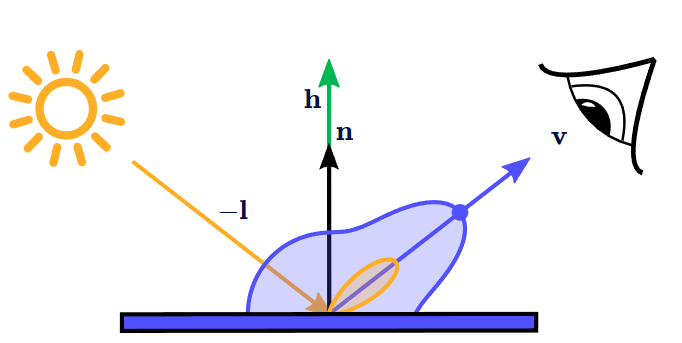
\includegraphics[width=0.95\textwidth, align=b]{Plantilla-TFG-master/img/phong1.png}
     \end{minipage}
     \begin{minipage}[c]{0.32\linewidth}
        \centering
        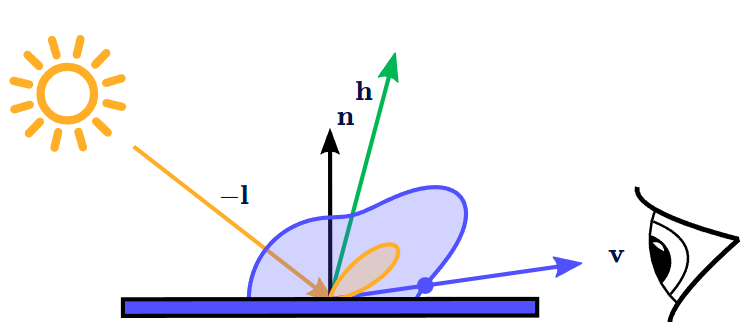
\includegraphics[width=0.95\textwidth, align=b]{Plantilla-TFG-master/img/phong2.png}
     \end{minipage}
     \begin{minipage}[c]{0.32\linewidth}
        \centering
        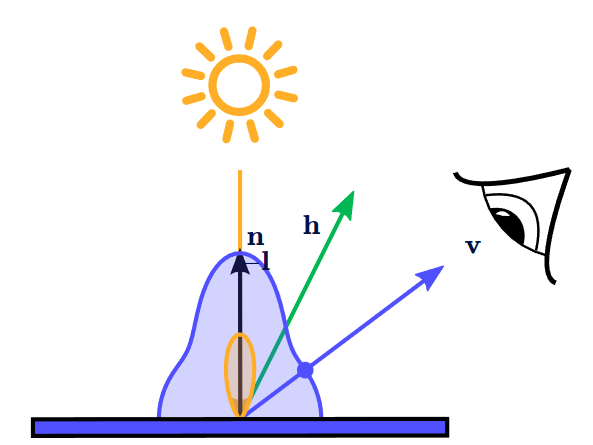
\includegraphics[width=0.95\textwidth, align=b]{Plantilla-TFG-master/img/phong3.png}
     \end{minipage}
     \caption{Comportamiento de  $h_m$ con $\Vert R_S\Vert =\Vert R_D\Vert$}
     \label{fig:phong}
\end{figure}

Aunque esta nueva versión se trate de una simplificación del modelo de Phong, lo cierto es que produce resultados más convincentes que este. En particular, mientras que el modelo de Blinn siempre produce brillos redondos en superficies planas, el de Blinn-Phong los genera con una forma más elíptica cuando se observa la superficie desde un ángulo acusado, como se observa en la \autoref{fig:difBlinn}. 
\begin{figure}[!h]
     \begin{minipage}[c]{0.49\linewidth}
        \centering
        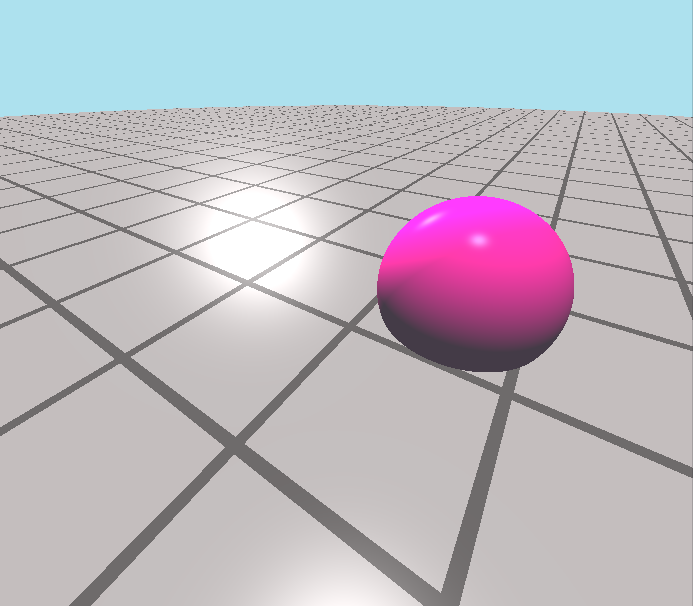
\includegraphics[width=0.9\textwidth]{Plantilla-TFG-master/img/compB.png}
        \caption{Phong}
     \end{minipage}
     \begin{minipage}[c]{0.49\linewidth}
        \centering
        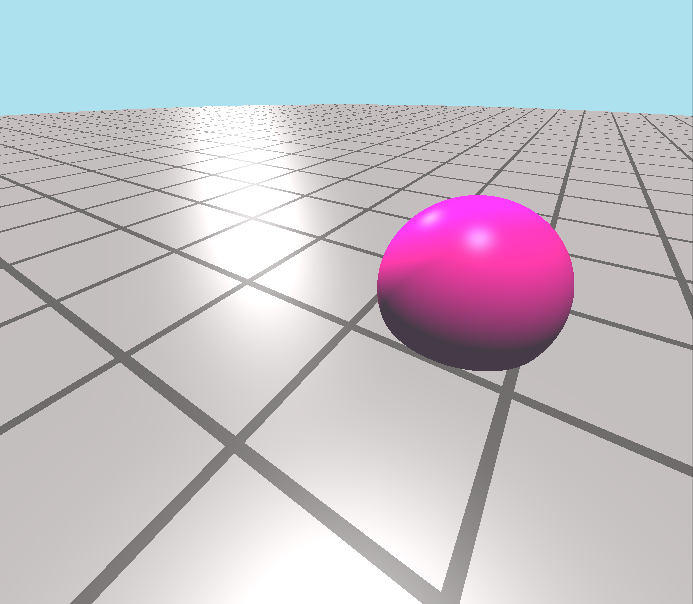
\includegraphics[width=0.9\textwidth]{Plantilla-TFG-master/img/compBP.png}
        \caption{Blinn-Phong}
     \end{minipage}
     \caption{Zonas brillantes en modelos de Phong y Blinn-Phong}
     \label{fig:difBlinn}
\end{figure}

\begin{definicion}[Modelo de Blinn-Phong]
    En el contexto de la \autoref{def:blinn}, la radiancia percibida en el punto $p\in\R^3$ desde la dirección $v\in\R^3$ con $\Vert v \Vert = 1$ según el modelo de Blinn-Phong viene dada por
    \begin{equation*}
        L(p,v) = L_A+L_E+ \sum_{i=0}^n S_i \Bigg[ R_A + R_E\cdot \left(N_p\cdot \frac{l_i + v}{\Vert l_i + v\Vert} \right)^{\alpha} + R_D\cdot \Max(0,l_i\cdot N_p) \Bigg].
    \end{equation*}
\end{definicion}

Ya podemos darle forma a las funciones \texttt{DibujarSuperficie} y \texttt{DibujarFondo} usadas en la \autoref{a:spheretracing}, suponiendo que pasamos como \textit{uniforms} los parámetros del material y los valores $l_i$ y $S_i$ para cada $i\in \{1,\dots, n\}$.
\begin{figure}[ht!]
    \centering
    
       \begin{algorithm}[H]
            \caption{DibujarSupercicie}
                \KwData{punto $p$, dirección del rayo $v$, distancia $\phi(p)$}
                \KwResult{terna RGB con la radiancia percibida en el punto $p$}
                $L \gets L_A$ \Comment{Radiancia final}
                \For{$i \in \{1,\dots, n\}$} {

                    
                    $h \gets normalizar(L_i - v)$ \Comment{Observador en dirección opuesta a la del rayo}
                    
                    $N_p \gets$ CalcularNormal$(p)$
                    
                    $NLi \gets \Max(0,\ N_p\cdot l_i)$
                    
                    $NH \gets \Max(0,\ N_p \cdot h)$\newline

                    $f_{ra} = R_A$
                    
                    $f_{rd} = NLi\cdot R_D$
                    
                    $f_{re} = NLi \cdot R_E \cdot NH^{\alpha}$\newline

                    $L \gets L + S_i\cdot (f_{ra} + f_{rd} + f_{re})$
                }

                \Return{$L$}
        \end{algorithm}
    \begin{algorithm}[H]
            \caption{DibujarFondo}
                \KwResult{terna RGB con el color de fondo de la escena}
                \Return{$L_A$}
        \end{algorithm}

        \caption{Implementación de las funciones \texttt{DibujarSuperficie} y \texttt{DibujarFondo}}
\end{figure}
Solo queda un asunto por tratar. A la vista de la expresión de $f_r$ \eqref{eq:fr} y del código anterior, somos capaces de calcular todos los valores a excepción de uno, el del vector normal. En la siguiente sección veremos presentamos una técnica para calcularlo de forma aproximada. 
